% !TeX spellcheck = en_US
% !TeX root = ../BachelorThesis.tex

\section{Sleep Duration}
In this section we take a look at the sleep duration.
As we can see in \Cref{table: Sleep Analysis}, there are a lot of day ratings without a measurement of sleep duration and vice versa. 
Another thing is that there can be multiple entries that have the same date but a different sleep duration.
This is only the case for the devices that resulted in the data shown in \Cref{table:sleepduration1} and \Cref{table:sleepduration2}.
These `splits' occur when a person's sleep is interrupted. 
A sleep interruption is detected by the device, which then saves the new measurement as a separate one.
Some participants also took one or more naps during the day, resulting in more entries with the same data. 
For dates without a sleep measurement, the format is Y-M-D.
For dates with one or multiple measurements, the date is formatted as Y-M-D H-M-S.
This latter date format indicates the time the person stopped sleeping and awakened.
Due to this formatting, we can distinguish if an interruption belongs to the previous or the current night.
For the used devices that resulted in the measurements in \Cref{table:sleepduration3} and \Cref{table:sleepduration4}, the sleep durations are never split.
The API returned the total sleep duration of that day.
The dates in these measurements only show the day the measurement belongs to and do not indicate the time at which the participant fell asleep or awakened.
For analysis, splits belonging to the same day were summed and represented the total sleep duration for that day.
Looking at \Cref{table: Sleep Analysis}, it is strange that a lot of values are missing. 
Especially in \Cref{table:sleepduration1}, we see a lot of measurements where the time of awakening is around 5 in the morning. 
We would expect that this is due to an interruption and that the person would resume his sleep.
This is however not confirmed by the data, because in most of these cases there is no additional entry for that specific date.
It could also be possible that this particular participant decided to take of his wristband during the night because it was becoming too uncomfortable.
Another explanation could be that a couple of hours before awakening, people reside in a sleep stage from which it is easier to awake and also involves more movement.
Due to this increased amount of movement, the device could classify your sleep state as `not sleeping', although you are. 
For dates with no measurements, it might be the case that the participant decided not to wear the activity tracker at all.
%
\newpage
\begin{table}[H]
	\centering
	\begin{tabular}{@{}lll@{}}
		\toprule
		\textbf{Participant} & \bm{$\tau$} & \bm{$p$}\\
		\midrule
		\subref{fig: sleep user1} & $0.426694$ & $0.042305$ \\
		\subref{fig: sleep user2} & $0.188608$ & $0.447772$ \\
		\subref{fig: sleep user3} & $0.070367$ & $0.558409$ \\
		\subref{fig: sleep user4} & $0.051105$ & $0.686289$  \\ 
		\bottomrule
	\end{tabular}
	\captionof{table}{Expressing the rank correlation between sleep duration and day rating.}
	\label{table:sleep duration test kendall tau}
\end{table}
%
\begin{figure}[H]
	\centering
	\subfloat[]{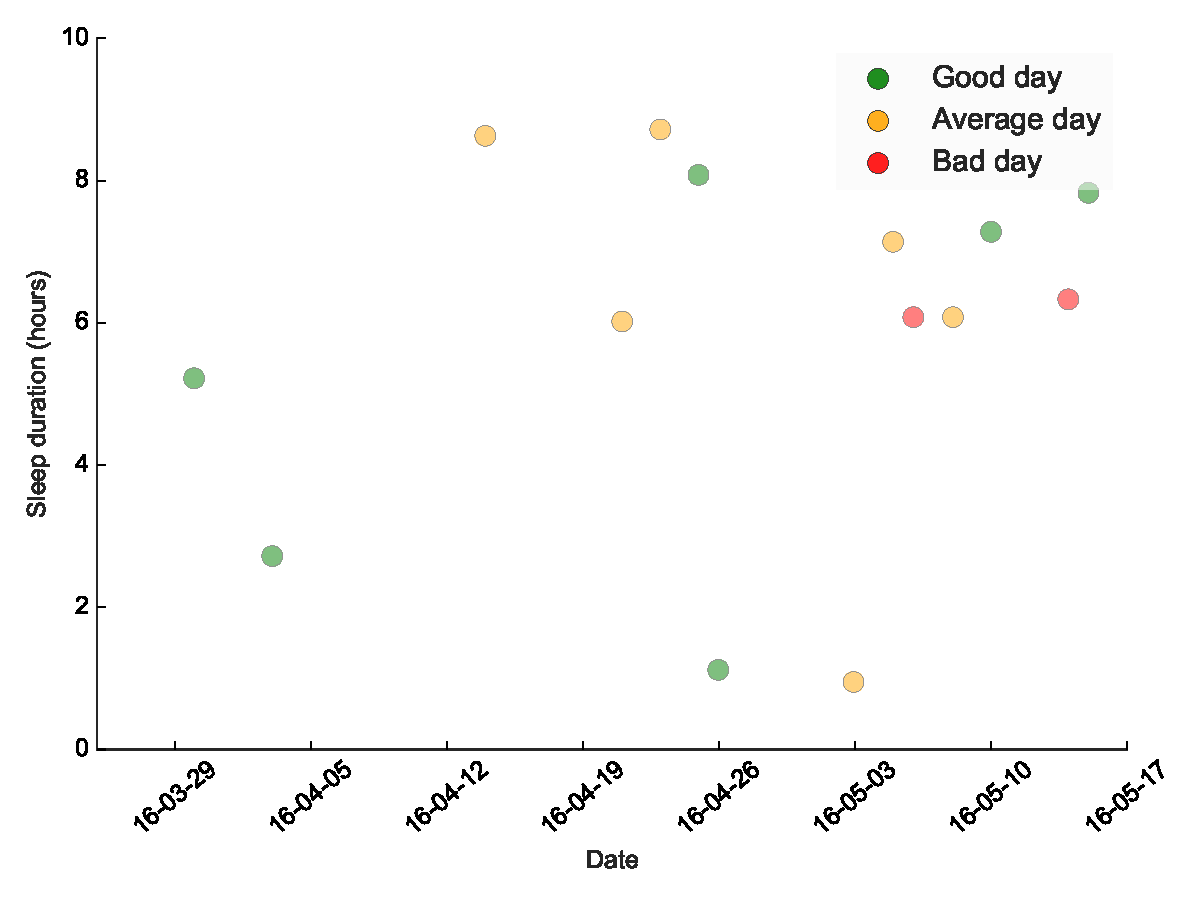
\includegraphics[scale=0.29]{img/sleep/2Dy2uFf3aw6jv9r5u}
		\label{fig: sleep user1}
	}
	\hspace{0.5cm}
	\subfloat[]{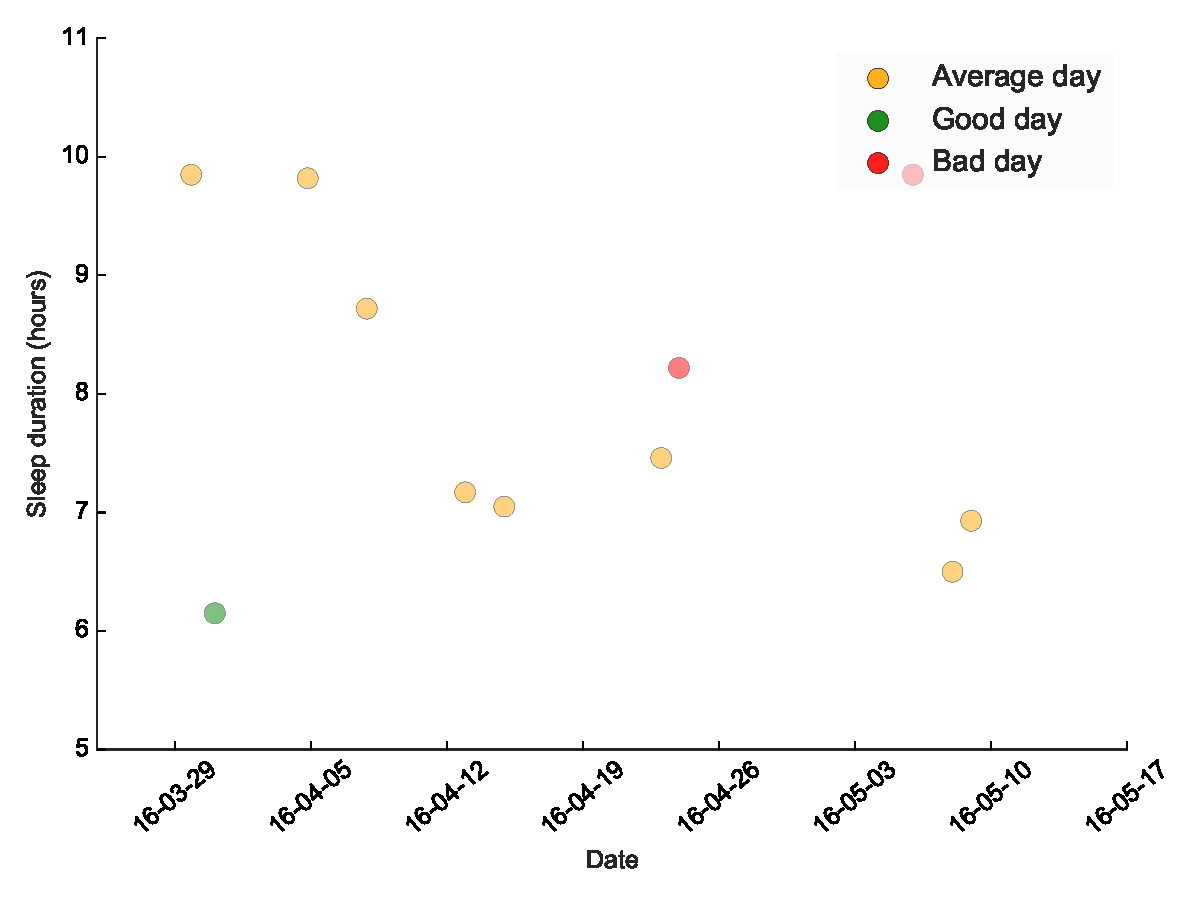
\includegraphics[scale=0.29]{img/sleep/dW4YzJQEaidmyhsuY}
		\label{fig: sleep user2}
	}
	\vfill
	\subfloat[]{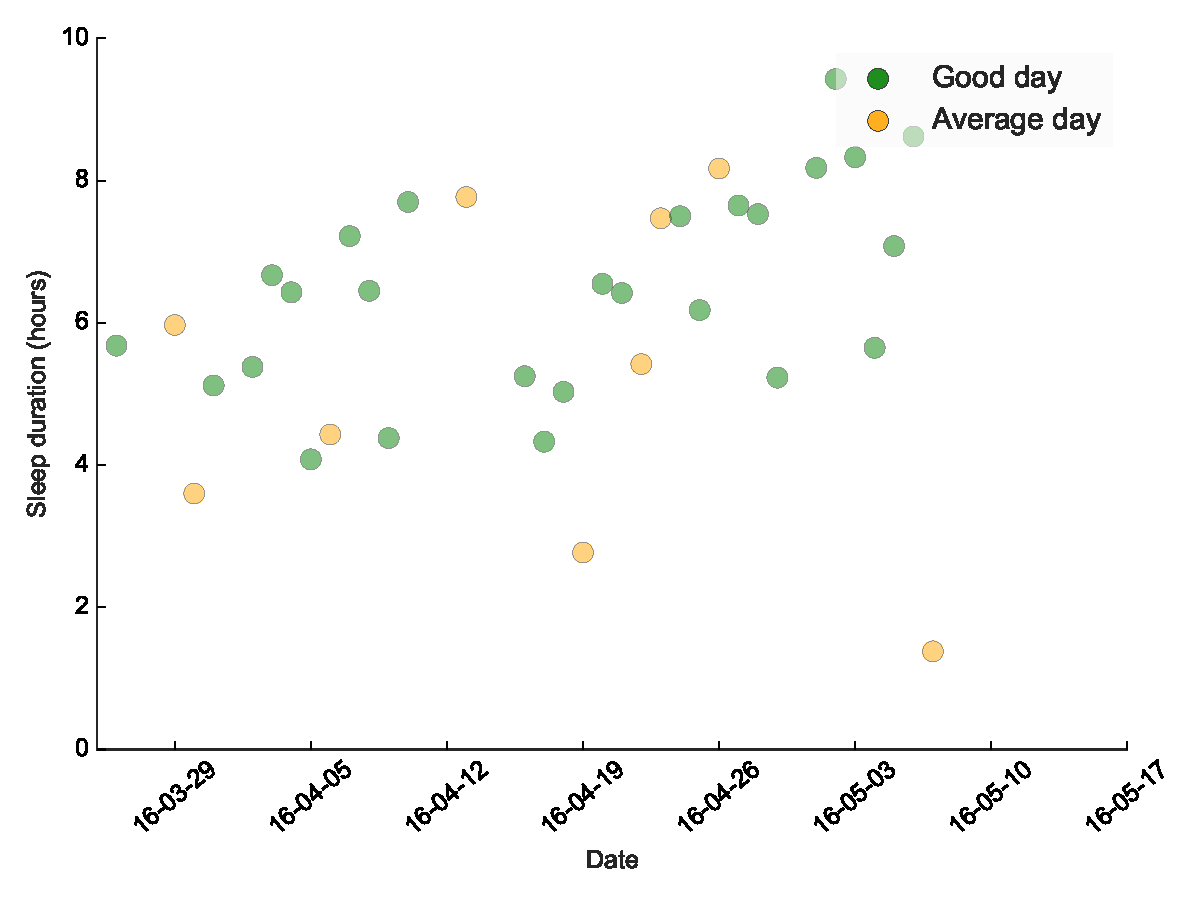
\includegraphics[scale=0.29]{img/sleep/gGSWzh5PnqgFdCpq4}
		\label{fig: sleep user3}
	}
	\hspace{0.5cm}
	\subfloat[]{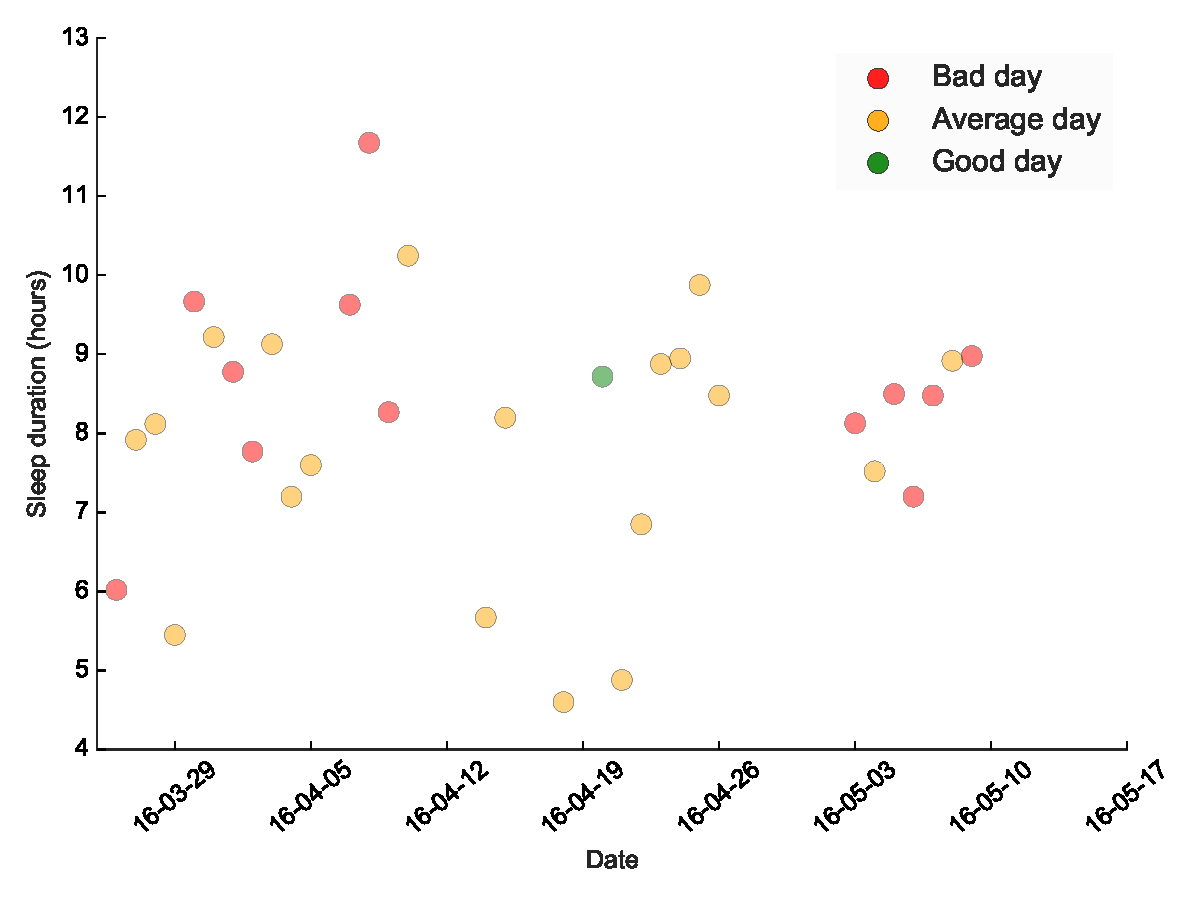
\includegraphics[scale=0.29]{img/sleep/S2usWtx8WXPe8S88r}
		\label{fig: sleep user4}
	}
	\captionof{figure}{Plots of the sleep durations of the participants. 
		Only dates that both had a rating and a measurement of the sleep duration are shown.
		As can be seen in the legend of each of the figures, each point is colored according to the rating given by the participant for that day.}
	\label{fig: sleep duration analysis}
\end{figure}
\newpage
%
In \Cref{fig: sleep duration analysis}, we see the plots for each of the participant.
The corresponding coefficients are shown in \Cref{table:sleep duration test kendall tau}.
Looking at these coefficients, we see that all of them are smaller than $0.5$ and have a positive sign.
In fact, most of them have a value that is close to zero.
For participant \subref{fig: sleep user3} and \subref{fig: sleep user4}, the coefficient is very small.
Although a bit bigger, the same applies for the value of the coefficient for participant \subref{fig: sleep user2}.
The coefficient for participant \subref{fig: sleep user1} is the biggest.
Because most values of the coefficients are low, they suggest that the measurement and the rating of the next day are statistically independent.
Only for participant \subref{fig: sleep user1}, the $p$-value is significant.
For all the other entries, there are no significant $p$-values.
In some of the figures, we see some measurements that have a total sleep duration of less than 4 hours.
Although this is possible, it is not very likely. 
We could add an extra survey to specifically ask for the quality of the night, so that we can verify our measurements against these answers (triangulation).
This could also include a question where the participant can give an indication of the total sleep he or she had during the night. 
Using these extra questions, we could determine more easily if the measurements are reliable or not.